\section{Future Works}

\begin{itemize}

\item There are some limitations in the process of constructing the RAT table. One major limitation is that swapping is not allowed more than once for an entry. Thus there can be a maximum of 128 swaps for a single Lookup table. To allow more number of swaps per entry, more sophisticated data structure is required.

\item The big picture that summarises the performance difference with the straightforward Table lookup approach is given below

\begin{center}
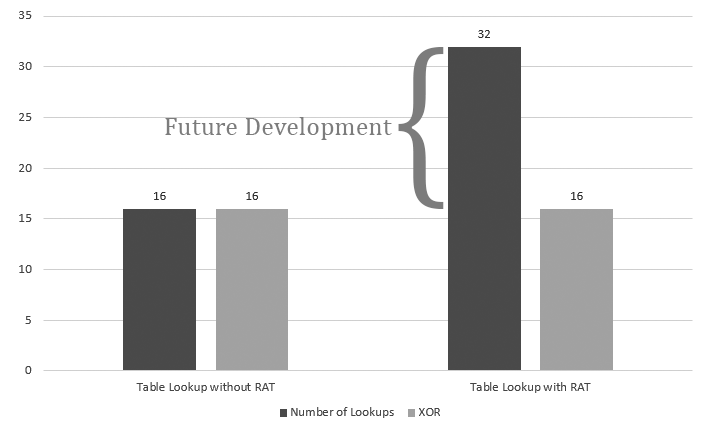
\includegraphics[scale=0.4,natwidth=713,natheight=436]{Figures/performance.png}
\captionof{figure}{Comparison with straightforward Table Lookup approach.}
\label{fig: Comparison with straightforward Table Lookup approach.}
\end{center}

As we can see, we need 2 times more table lookups than the ordinary approach. The area of future development is to reduce this factor.

\item Another big concern is that, RAT tables add a fair amount of memory overhead to the encrypting process. Whereas the Lookup tables altogether require 4KB of space, RAT tables requires 1KB of space. Although not a big figure to worry about, space overhead can be reduced with the assistance of some more tables of smaller sizes.

\end{itemize}
